\secrel{Пакет Maxima}\secdown

\prog{Maxima}\ -- пакет CAS символьной математики.

\bigskip\noindent
\begin{tabular}{p{0.25\textwidth} p{0.75\textwidth}}
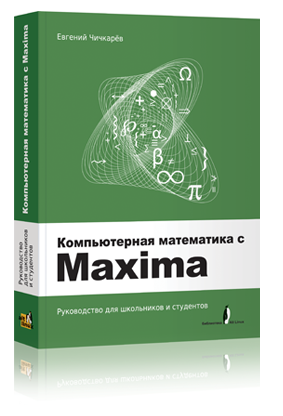
\includegraphics[height=0.45\textheight]{math/maxima/BookMaxima.png}
&
\parbox[b]{0.7\textwidth}{
Евгений Чичкарёв\\
\textbf{Компьютерная математика с Maxima. Руководство для школьников и
студентов}\\
\url{http://www.altlinux.org/Books:Maxima}\\
}
\\
\end{tabular}

\bigskip
Дополнительная документация:
\url{http://maxima.sourceforge.net/ru/documentation.html}

\bigskip\noindent
\href{https://drive.google.com/file/d/0B0u4WeMjO894M01wZmNkSW9GRHM/view?usp=sharing}{PDF}\
для книги Ильина В.А., Силаев П.К. Система аналитических вычислений Maxima для
физиков-теоретиков\ \cite{maxphis}\ получена из файла \file{.ps}\ с помощью
сервиса \url{http://ps2pdf.com/convert.htm}.

\secrel{Установка Maxima под \win}

\menu{\winr>\url{http://maxima.sourceforge.net/ru/}>Загрузка}

\menu{Maxima-Windows>\file{5.34.1-Windows}>\file{maxima-5.34.1.exe}}

\menu{\file{maxima-5.34.1.exe}>Установка>Язык>\textbf{English}>OK>Next}

\menu{License>I accept>Next>}

\menu{Install folder>по умолчанию>Next}

\menu{Components>\uncheckbox\ Language packs>Next>Next}

\menu{\checkbox\ wxMaxima>\uncheckbox\ XMaxima>Next>Install>Next>Finish}

\menu{\winstart>Maxima-5.34.1>wxMaxima>\rms>Закрепить в панели задач}

\secup
